\hypertarget{gIMRPhenomD_8cpp}{}\section{src/g\+I\+M\+R\+PhenomD.cpp File Reference}
\label{gIMRPhenomD_8cpp}\index{src/g\+I\+M\+R\+Phenom\+D.\+cpp@{src/g\+I\+M\+R\+Phenom\+D.\+cpp}}
{\ttfamily \#include \char`\"{}g\+I\+M\+R\+Phenom\+D.\+h\char`\"{}}\newline
{\ttfamily \#include \char`\"{}util.\+h\char`\"{}}\newline
{\ttfamily \#include \char`\"{}I\+M\+R\+Phenom\+D.\+h\char`\"{}}\newline
{\ttfamily \#include $<$adolc/adouble.\+h$>$}\newline
Include dependency graph for g\+I\+M\+R\+Phenom\+D.\+cpp\+:\nopagebreak
\begin{figure}[H]
\begin{center}
\leavevmode
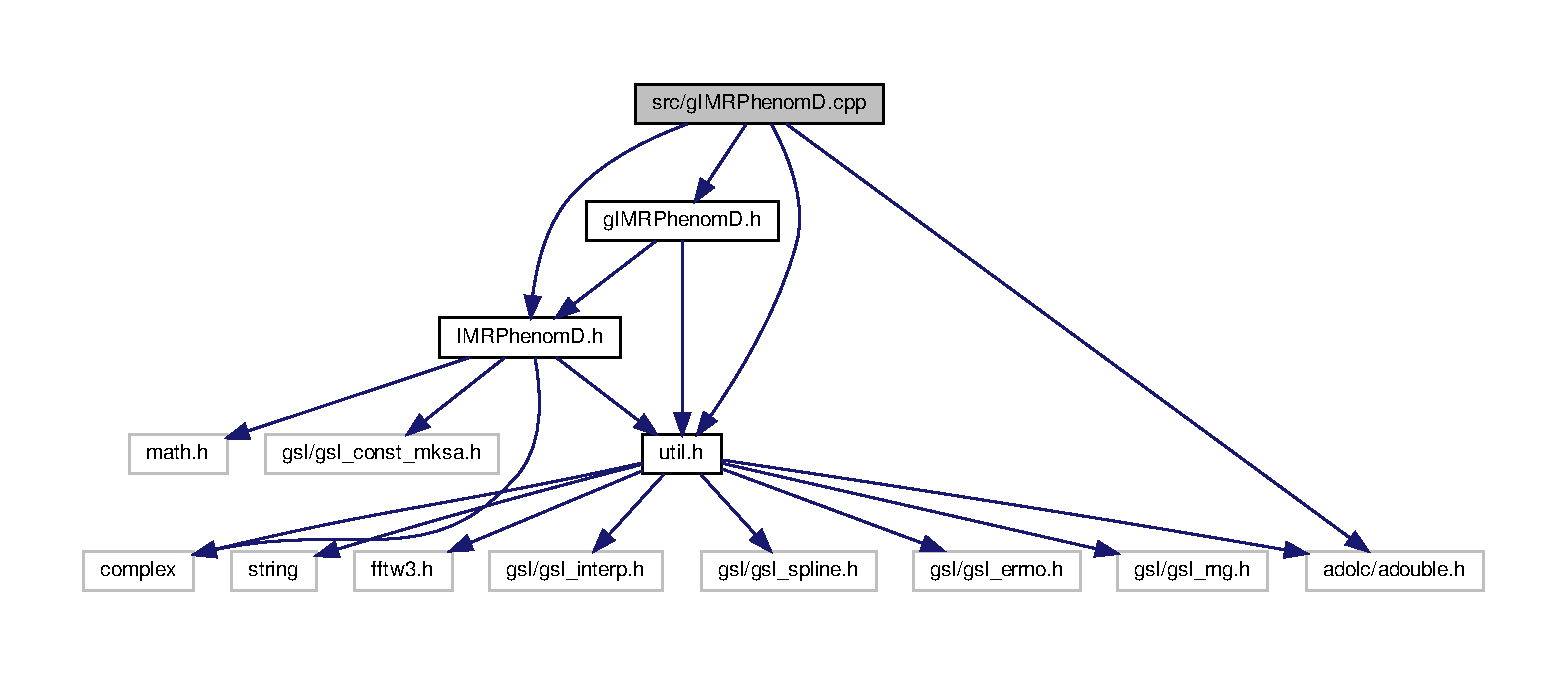
\includegraphics[width=350pt]{gIMRPhenomD_8cpp__incl}
\end{center}
\end{figure}


\subsection{Detailed Description}
g\+I\+MR parameterization for modifications to GR

four groups -- phi, beta, sigma, alpha

beta can be 2,3

alpha can be 2,3,4

sigma can be 2,3,4

phi can be -\/4-\/9 (8, 9 correspond to the logarithmic terms at 5 and 6) 